\chapter{Experimental Study}
\label{chp:exp}


To test and support our theoretical approach to compute spatial alarms in the obstructed space efficiently, we have done extensive experiments using both real and synthetic data-sets. In this chapter, we are going to present the validation and comparison of the proposed approach against the naive approach regarding various effective parameters
\section{\label{sec:exp}Experiment Setup}
In this section, the detailed setup of the experiments is described as per the following sub-sections
\subsection{Data Set Used}

We have used both real and synthetic data-sets  to evaluate our solution. In case of real data-sets, we have used obstacles and point of interests (POIs) of Germany \cite{Germany}. The obstacle set has 30674 minimum bounded rectangles (MBRs) of railway lines (rrlines). In our experiment, we assume obstacles to be presented by MBRs, but our algorithm can handle any type of obstacles. The POI set has 76999 MBRs of hypsography data (hypsogr). We assume data-points to be endpoints of the hypsography data. In this way, the POIs and obstacles are in the same plane which allows us to simulate a real-life scenario. We do not allow intersections between POIs and obstacles, neither do we allow duplicate POIs or obstacles. In case of synthetic data-sets, we have generated the obstacles and POIs from the real datasets following a uniform distribution. Before using in the real experiment, we have always normalized both real and synthetic dataset in a $  10,000 \times 10,000 $ grid.\\
In our experiments, we have assumed only one type of POIs. However, our approach also can handle multiple types of POI. \\
Prior to  running the main algorithms, two separate R-trees are built to store the POIs and the obstacles respectively from the used data-sets.\\





\subsection{Sample Query Generation}
We have simulated the movement of the client randomly in the runtime. During the experiments, we have assumed that any movement-path of the client can be synthesized as piecewise-linear, i.e., a set of directed straight lines. In the explicit form of any straight line, $ y=mx+c$ , for any client position (x, y), we have randomized the slope m giving some value of c each time. The direction of the client along this new straight line is also randomized to be either in forward or backward along the path, with a bias towards the forward direction, as the real world user-movement with a definite source and destination usually proposes.\\
After determining the client’s new position along this path, in the naive approach, the algorithm 1 directly queries the server for POIs and obstacles within the client’s alarming range. Alternately, in the main approach, the algorithm 6 checks the region-crosses and queries the server if necessary.\\
The client’s velocity is also randomized within a certain range to give a new position of the client along the current direction in the next iteration, which again generates a new server-query accordingly.\\
Meanwhile, the direction of the client is predicted in the main approach from the latest set of piecewise linear paths in the client’s movement history. This prediction procedure has already been described in the  Algorithm section.\\

\subsection{Measurement of the Performance Parameters}
In our experiments, we vary the following query parameters:\\ (i) Clients Velocity Range\\ (ii) the Alarm Range r\\ (iii) the size of data sets (synthetic data set)\\. Table ~\ref{table:exp_setup} summarizes the parameter values used in our experiments. In all experiments, we estimate I/O accesses and the query processing time to measure the efficiency of our algorithms. In each set of experiments, we run the experiment for 100 queries and present the average result.
\vspace*{10pt}
\begin{table}[htbp]
  \centering

\begin{tabular}{|c|c|c|}  \hline
 %after \\: \hline or \cline{col1-col2} \cline{col3-col4} ...
  Parameter& Values & Default\\
  \hline
  Client’s Movement lenght($ v $) Range (Unit) & 500,1000,1500,2000 &2000 \\
  \hline
  Alarm Range $r$& 60, 80, 100, 150 &150\\
  \hline
  Synthetic data set size & 5K, 7K, 15K, 38K & - \\
  \hline
\end{tabular}
\caption{Values of different query parameters used in our experiments} \label{table:exp_setup} \vspace{-2mm}
\end{table}


\subsection{Implementation Language and Tools}
The project of our experiment is implemented using C++ language and have been compiled, debugged and tested using Microsoft Visual Studio 2015 Enterprise edition with a full version student-license from DreamSpark.

\subsection{PC Configuration}
We have run our experiments in three PCs of the following configurations:\\
1. Intel Core i5 2.9 GHz (Quad Core), 12 GB RAM \\
2. Intel Core i5 2.3 GHz (Quad Core), 4 GB RAM \\
3. AMD FX 6100 3.3 GHz (Hexa Core), 8 GB RAM \\
The average of these multiple runs is taken to measure and compare the performance of both the naïve approach and our approach.


In Section~\ref{subsec:naive}, we compare the results of two approaches.


\subsection{Comparison of Our Approach with Naive Aproach}
\label{subsec:naive}
%%TO DO :Write our naive approach experiment evaluation here
%In this section, we present the experimental results for processing $k$GTP queries for aggregate function SUM. For SUM, we name our proposed approach and the naive approach as $kGTPQ_{sum}$ and $kGTPQ-NA_{sum}$, respectively. In the following sets of experiments, we vary group size, the answer set size, query area, and dataset size. When we vary one parameter, we set other parameters to default values as stated in Table~\ref{table:exp_setup}.
\textbf{\emph{Effect of Clients movement length: }}Figure~\ref{graph:ClientVelocity}(a) \ref{graph:ClientVelocity}(b)\ref{graph:ClientVelocity}(c) and \ref{graph:ClientVelocity}(d) show processing time,server query, i/o (obstacle) and i/o(POI) respectively, for processing spatial alarm queries using naive approach and our approach. We observe that for both algorithms processing time and server query increase with the increase in length of user's movement. We also observe that in terms of server query our approach performs almost 14times better than the naive approach. and incase of runtime our approach runs almost 3 times better than the naive approach. Incase of I/o our approach initially is higher than the naive approach but, in the average case our approach is better than the naive approach by approximately 10 times.

\vspace*{10pt}

\begin{figure}[htbp]
 \vspace{-2mm}
  \begin{center}
    \begin{tabular}{cc}
        \hspace{-5mm}
     \resizebox{70mm}{!}{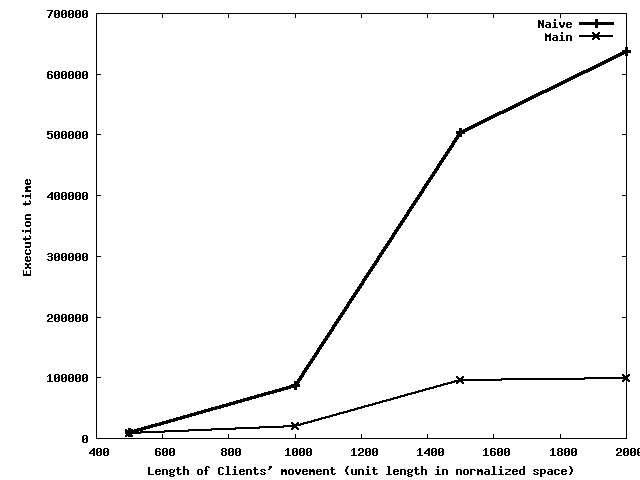
\includegraphics[]{exec_l.png}} &
        \hspace{-5mm}
         \vspace{-2mm}
      \resizebox{70mm}{!}{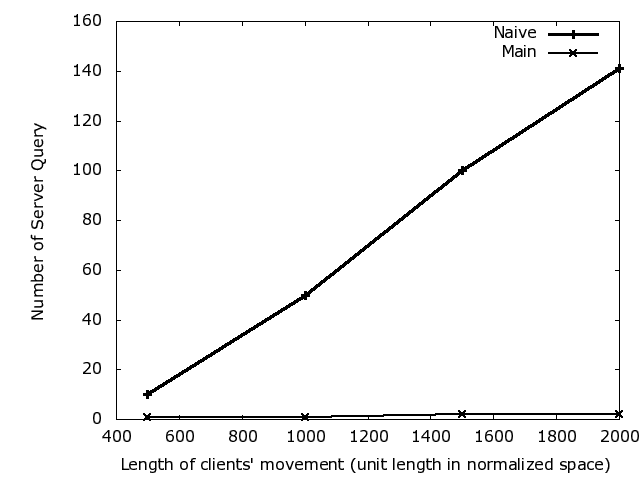
\includegraphics[]{server_l.png}} \\
    \scriptsize{(a) \textsc{}\hspace{0mm}} & \scriptsize{(b) \textsc{}}\\
       \hspace{-5mm}
      \resizebox{70mm}{!}{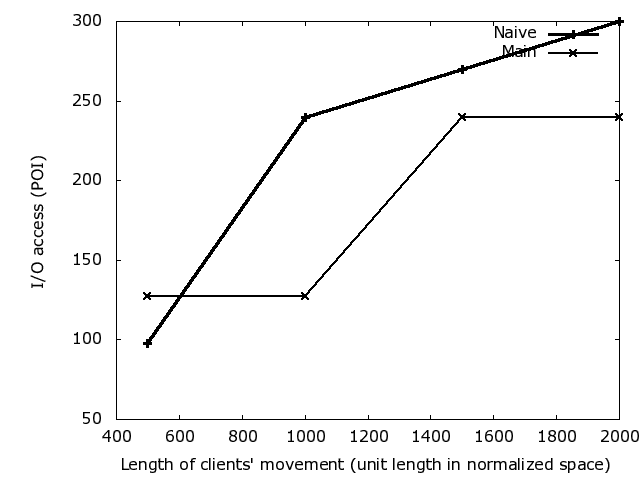
\includegraphics{io_l.png}} &
        \hspace{-5mm}
     \resizebox{70mm}{!}{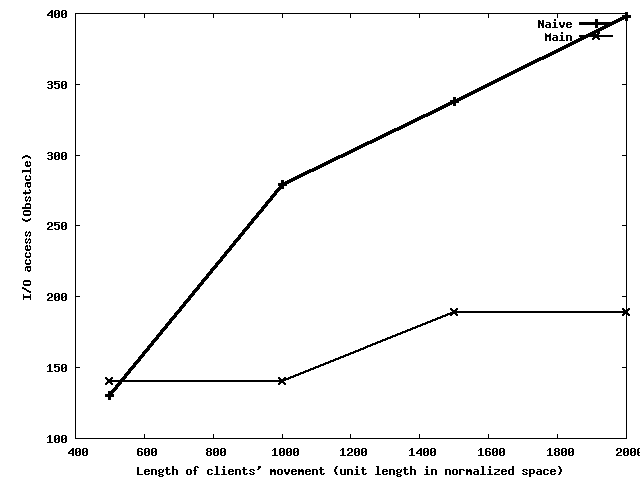
\includegraphics{io_l_obs.png}} \\
     \scriptsize{(c) \hspace{0mm}} & \scriptsize{(d) }\\
     \hspace{-5mm}
%      \resizebox{40mm}{!}{\includegraphics{graph/sum/vk_answer.pdf}} &
%        \hspace{-5mm}
%      \resizebox{40mm}{!}{\includegraphics{graph/max/vk_answer.pdf}} \\
%       \scriptsize{(e) \textsc{sum}\hspace{0mm}} & \scriptsize{(f) \textsc{max}}
        \end{tabular}
    \caption{Effect of Client's movement length  for Germany data  (a) query processing time and (b) Server Query (c) IO-POI (d) IO-obstacle}
    \label{graph:ClientVelocity}
  \end{center}
 %  \vspace{-6mm}
\end{figure}
\textbf{\emph{Effect of Alarm range $r$: }}
\ref{graph:Alarm Range}(b)\ref{graph:Alarm Range}(c) and \ref{graph:Alarm Range}(d) show processing time,server query, i/o (obstacle) and i/o(POI) respectively, for processing spatial alarm queries using naive approach and our approach. We observe that for both algorithms processing time and server query increase with the increase in length of alarm range. We also observe that in every alarm range our approach outperforms the naive approach by multiple times.
%\vspace*{10pt}
%\textbf{\emph{Effect of answer set $k$: }} In this set of experiments, we vary $k$ as 2, 4, 8, and 16, and compare the experimental results $kGTPQ_{sum}$ and $kGTPQ-NA_{sum}$.


%From Figure ~\ref{graph:sum_k}(a) and Figure~\ref{graph:sum_k}(b), we observe that I/Os and processing time increase with the increase of $k$ for both $kGTPQ_{sum}$ and $kGTPQ-NA_{sum}$. Figures show that $kGTPQ-NA_{sum}$ takes almost one and half orders of magnitude more I/Os compared to $kGTPQ_{sum}$. We also see from Figure~\ref{graph:sum_k}(b) that the query processing time of $kGTPQ-NA_{sum}$ is on average one and
%half orders of magnitude higher than that of $kGTPQ_{sum}$. The superiority of our approach over the naive approach comes from the ellipse based pruning strategies that reduces the search space significantly.

\vspace*{10pt}

\begin{figure}[htbp]
 \vspace{-2mm}
 \begin{center}
   \begin{tabular}{cc}
        \hspace{-5mm}
     \resizebox{70mm}{!}{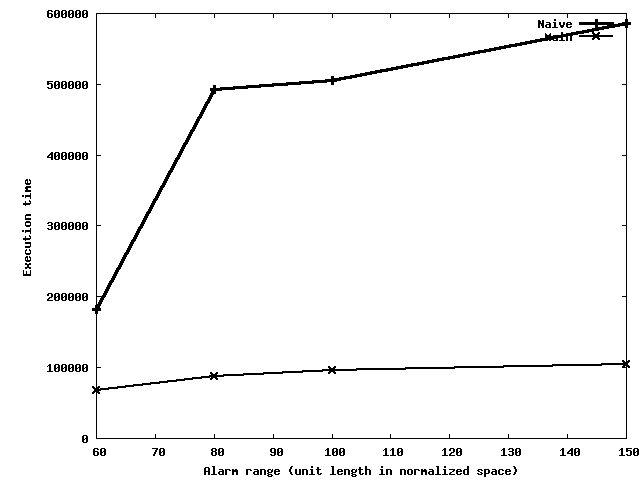
\includegraphics[]{exec_alarm.png}} &
        \hspace{-5mm}
         \vspace{-2mm}
      \resizebox{70mm}{!}{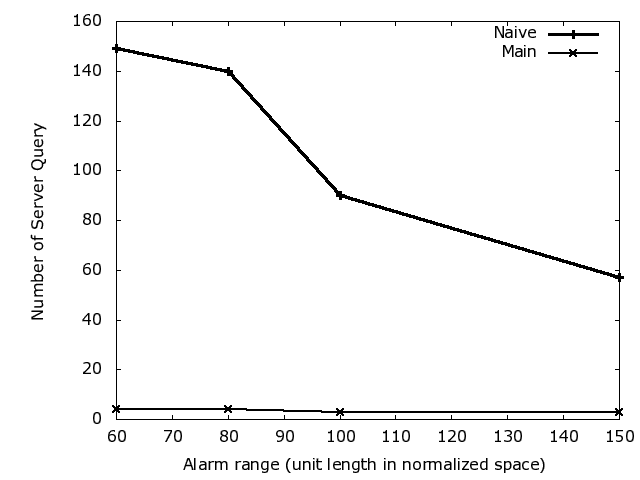
\includegraphics[]{server_alarm.png}} \\
     \scriptsize{(a) \textsc{}\hspace{0mm}} & \scriptsize{(b) \textsc{}}\\
       \hspace{-5mm}
       \resizebox{70mm}{!}{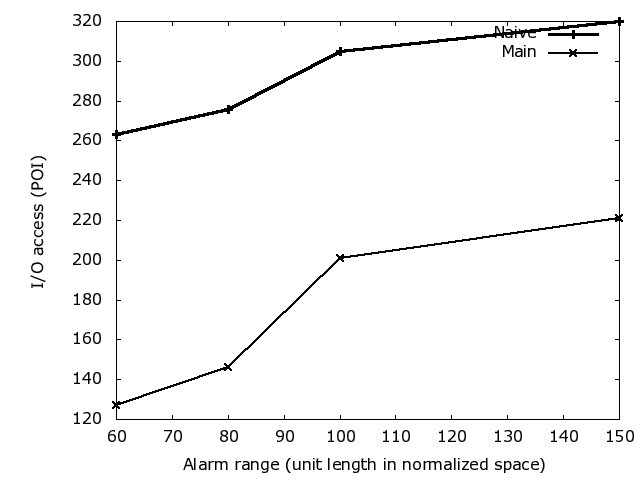
\includegraphics{io_r.png}} &
        \hspace{-5mm}
     \resizebox{70mm}{!}{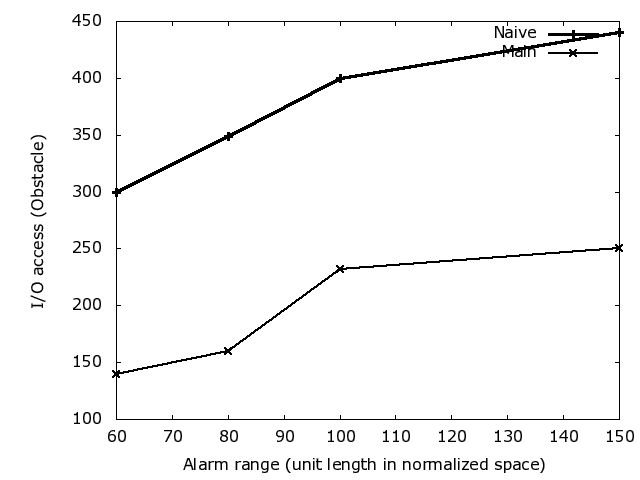
\includegraphics{io_r_obs.png}} \\
     \scriptsize{(c) \hspace{0mm}} & \scriptsize{(d) }\\
      \hspace{-5mm}
%      \resizebox{40mm}{!}{\includegraphics{graph/sum/vk_answer.pdf}} &
%        \hspace{-5mm}
%      \resizebox{40mm}{!}{\includegraphics{graph/max/vk_answer.pdf}} \\
%       \scriptsize{(e) \textsc{sum}\hspace{0mm}} & \scriptsize{(f) \textsc{max}}
        \end{tabular}
    \caption{Effect of Alarm Range $r$  for Germany data  (a) query processing time ,(b) Server Query ,(c) I/O(obstacle) and (d) I/O(POI)}
    \label{graph:Alarm Range}
  \end{center}
 %  \vspace{-6mm}
\end{figure}
%\vspace*{10pt}

%\textbf{\emph{Effect of Query Area $M$: }}In this case, we vary the query area $M$ as 2\%, 4\%, 8\% and 16\% of the data space. Figure~\ref{graph:sum_m}(a) and ~\ref{graph:sum_m}(b) show I/Os and query processing time, required by $kGTPQ_{sum}$ and $kGTPQ-NA_{sum}$, respectively. Since we need to access more data points from $R$-trees of different data types for a larger $M$, both I/Os and processing time increase with the increase of $M$ for both approaches.


%Figure~\ref{graph:sum_m}(a) shows that $kGTPQ-NA_{sum}$ requires at least one and half orders of
%magnitude more I/Os than that of $kGTPQ_{sum}$. Similarly, Figure ~\ref{graph:sum_m}(b)
%shows that the processing time of $kGTPQ-NA_{sum}$ is on average one order of magnitude higher
%than that of $kGTPQ_{sum}$.
\ref{graph:dataset}(b)\ref{graph:dataset}(c) and \ref{graph:dataset}(d) show processing time,server query, i/o (obstacle) and i/o(POI) respectively, for processing spatial alarm queries using naive approach and our approach. We observe that for both algorithms processing time and server query increase with the increase in the size of synthetic dataset. We use uniform distribution of real dataset to produce datasets of size 5k,7k,15k and 38k. We also observe that in every synthetic dataset size our approach outperforms the naive approach by multiple times.

\vspace*{10pt}

\begin{figure}[htbp]
 \vspace{-2mm}
  \begin{center}
    \begin{tabular}{cc}
         \hspace{-5mm}
      \resizebox{70mm}{!}{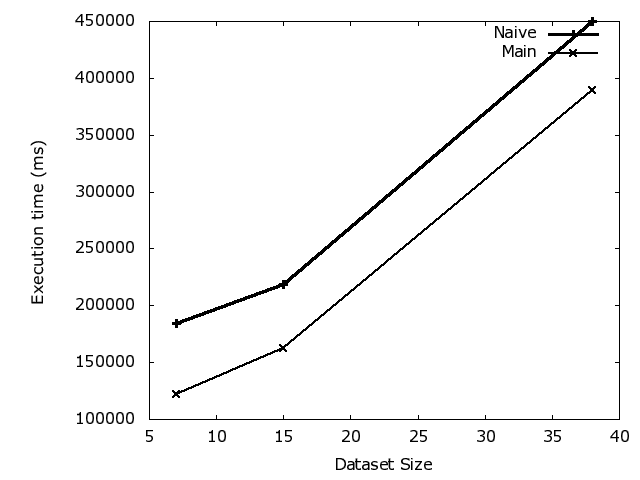
\includegraphics[]{exec_d.png}} &
       \hspace{-5mm}
         \vspace{-2mm}
    \resizebox{70mm}{!}{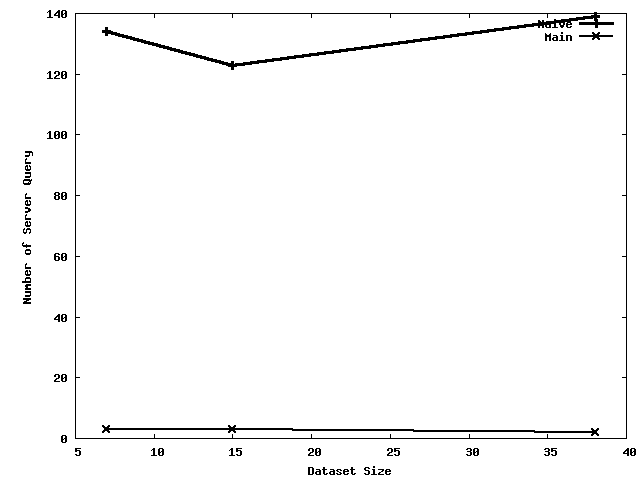
\includegraphics[]{server_d.png}} \\
     \scriptsize{(a) \textsc{}\hspace{0mm}} & \scriptsize{(b) \textsc{}}\\
        \hspace{-5mm}
      % \hspace{-5mm}
     \resizebox{70mm}{!}{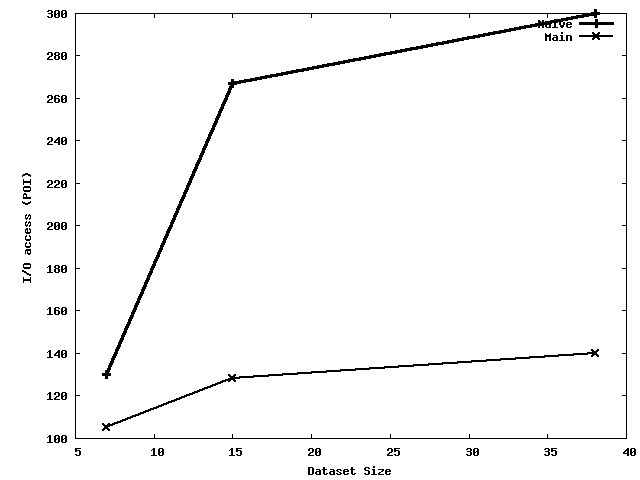
\includegraphics{io_d.png}} &
   
     \hspace{-5mm}
    \resizebox{70mm}{!}{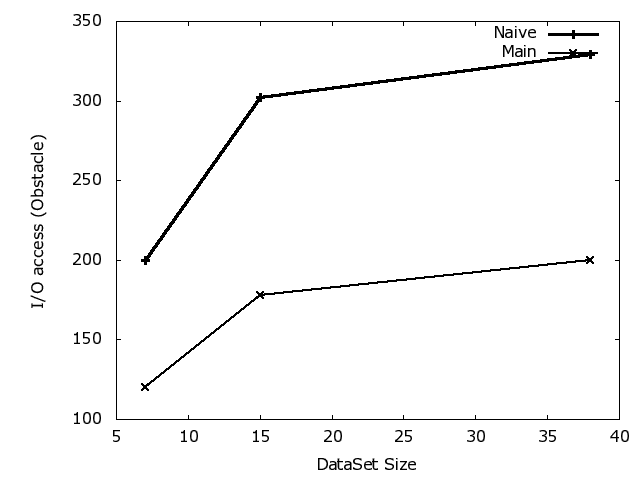
\includegraphics{io_d_obs.png}}\\
       \hspace{-5mm}
       \scriptsize{(c) \hspace{0mm}} & \scriptsize{(d) }\\
 %     \resizebox{40mm}{!}{\includegraphics{graph/max/vk_answer.pdf}} \\
  %     \scriptsize{(e) \textsc{sum}\hspace{0mm}} & \scriptsize{(f) \textsc{max}}
        \end{tabular}
    \caption{Effect of synthetic data set size  for Germany data (a) query processing time ,(b) Server Query ,(c) I/O(obstacle) and (d) I/O(POI)}
    \label{graph:dataset}
  \end{center}
   \vspace{-6mm}
\end{figure}
%\vspace*{10pt}


%\textbf{\emph{Effect of dataset size: }}In this set of experiments, we vary the road network size and number of POIs as stated in Table~\ref{table:exp_synthetic}. In this case, we use the first column, i.e., varying the number of nodes as 5000,
%10000,15000 and 20000 to identify four synthetic datasets. Figure~\ref{graph:sum_u}(a)
%and ~\ref{graph:sum_u}(b) show I/Os and processing time respectively for
%different synthetic dataset sizes. As expected, the experimental results show that




%\subsection{Our approach}
%\label{subsec:main}

\endinput 